%plurals_event
%PRECOMPILE COMMAND pdftex -ini -jobname="plurals_event_chap_34" "&pdflatex" mylatexformat.ltx plurals_event_chap_34.tex
\documentclass[english]{article}
\usepackage[T1]{fontenc}
\usepackage[latin1]{inputenc}
\usepackage[sort]{natbib}
\usepackage{stdprmbl}

\usepackage{parskip}

\lingset{interpartskip = -5pt}
\lingset{aboveexskip = 3pt,belowexskip = 3pt, belowpreambleskip = -3pt}

\definecolor{darkred}{rgb}{0.7,0,0}
\definecolor{blueish}{rgb}{0,0,0.7}
\newcommand{\ag}{\textsc{Agent}\xspace}
\newcommand{\thm}{\textsc{Theme}\xspace}
\newcommand{\goal}{\textsc{Goal}\xspace}

\newcommand{\fg}{\color{darkred}}
\newcommand{\bg}{\color{blueish}}


% \endofdump

\newcommand{\scale}{1}

\title{Plurals and events (chap. 9) : Cumulative quantification}
\author{Keny Chatain}

\begin{document}
\maketitle

This chapter is the grand finale I've eagerly been waiting for.

\section{Introduction}

\paragraph{The problem in a nutshell.}

In this section, Schein starts by outlining the problem of cumulative readings with modified numerals.

\pex
\a
Two detectives solved three crimes.
\a 
Less than two detectives solved less than 3 crimes. \label{detectives}
\xe
%
Schein notes that both sentences give rise to scopeless truth-conditions ; it isn't clear that either quantifier can be said to scope above the other. Despite this intuition, \clastxa can be given a logical representation in which one quantifier scopes above the other \cnextxa ; this is completely equivalent to a symmetrical logical representation where the opposite scope relation holds \cnextxb

\pex
\a 
$\exists X\in \textsf{2-detectives}, \exists Y\in \textsf{3-detectives},$ $X$ solved $Y$
\a
$\exists Y\in \textsf{3-detectives}, \exists X\in \textsf{2-detectives},$ $X$ solved $Y$
\xe
%
This fortunate scopelessness of the representation unfortunately does not hold for \cref{detectives}. Each gives rise to its own \emph{pseudo-cumulative} reading and neither reading are attested. We need a non-accidental way to generate scopelessness.

\pex
\a 
$<2\ X \in\textsf{detectives}, <3\ Y \in\textsf{crimes},$ $X$ solved $Y$\\
$\leftrightsquigarrow$\emph{the groups of detectives whose total crime score is less than 3 have less than 2 members}
\a 
$<3\ Y \in\textsf{crimes}, <2\ X \in\textsf{detectives}, $ $X$ solved $Y$
\xe
%
 Schein notes that this problem is not tied to assuming plural objects since his essentially equivalent LFs will also generate pseudo-cumulative reading.

\paragraph{The solution in a nutshell.} Schein proposes that at LF, the two quantifiers merge to form a binary object. The intended translation of these exotic LFs into logical formulas is in terms of an anaphoric dependency with two conjuncts

\pex
\a 
Less than two detectives reported less than 3 crimes to less than 2 agencies. 
\a 
\textbf{LF:}\\
%!TEX root = ../plurals_event_chap_9.tex
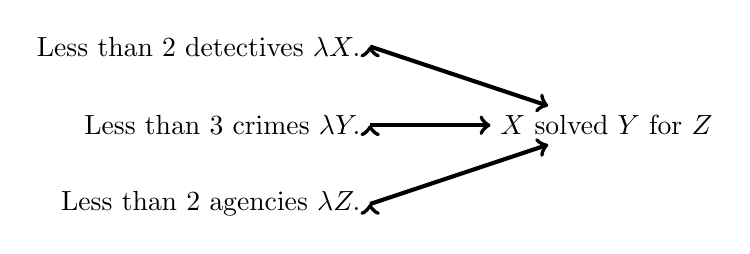
\begin{tikzpicture}[scale = \scale, baseline = {([yshift={-\ht\strutbox}]current bounding box.north)}]
\node[anchor = east] (v1) at (-3,1.5) {Less than 2 detectives $\lambda X.$};
\node[anchor = east] (v3) at (-3,0.5) {Less than 3 crimes $\lambda Y.$};
\node[anchor = east] (v4) at (-3,-0.5) {Less than 2 agencies $\lambda Z.$};
\node (v2) at (0,0.5) {$X$ solved $Y$ for $Z$};
\draw [->,line width = 1.5pt] (v1.east) edge (v2);
\draw [->, line width = 1.5pt] (v3.east) edge (v2);
\draw [->, line width = 1.5pt] (v4.east) edge (v2);
\end{tikzpicture}
\a \textbf{Logical formula:}\\
{\bg $[<2\ X \in\textsf{detectives}, \exists Y\in\textsf{crimes}, \exists Z\in\textsf{agencies},$\\
$\ag(E) = X \wedge \thm(E) = Y \wedge \goal(E) = Z \wedge \textsf{solved}(E)]^{73}$}\\[1ex]
{\fg $\wedge [\iota E: E = \text{pro}_{73},  <3\ Y\in\textsf{crimes}, \thm(E) = Y \wedge \textsf{solved}(E)]$\\
$\wedge [\iota E: E = \text{pro}_{73},  <3\ Z\in\textsf{agencies}, \goal(E) = Z \wedge \textsf{solved}(E)]$
}
\a \textbf{Schein's paraphrase:}\\
\emph{
Less than two detectives reported crimes to agencies\\
and there, less than 3 crimes were reported\\
and there, to less than 2 agencies were crimes reported
}
\xe
%
The logical formula has two parts: a {\bg conjunct} that introduces an antecedent ensemble event  which the subsequent {\fg conjuncts} further describe. In the subsequent section, Schein sets out to justify the exact shape of the logical formula he assumes:

\begin{itemize}
	\item \emph{Anaphora:} conjuncts related by anaphoric dependencies
	\item \emph{Cumulative asymmetry:} one quantifier is selected to belong to the clause that introduces the event referent
\end{itemize}
%
The event DR introduction is observed to follow the general rules of DR introduction ; it always introduce a maximal referent:


\section{Why cumulativity must be asymmetric}

This first section is devoted to justify the \emph{cumulative asymmetry}. This is a surprising feature of the analysis as the paraphrase of the truth conditions seem completely symmetric in the quantifiers that enter the relations:

\pex
\a 
Less than 3 detectives solved less than 5 crimes
\a \textbf{TCs:}\\
\emph{less than 3 detectives solved crimes}\\
\emph{less than 5 crimes were solved}
\xe
%
However, Schein wishes to suggest that the symmetric truth-conditions is inadequate for the more complex case in \cnextx:

\pex
\a 
Exactly two detectives each solved exactly two crimes for exactly 3 agencies
\a 
Exactly two detectives each solved exactly two crimes for exactly 1 agencies
\xe
%
The intended reading is one where:

\begin{itemize}
 	\item \emph{the crimes} is interpreted distributively relative to \emph{the detectives}
 	\item \emph{the detectives} and \emph{the agencies} enter a cumulative relation
 \end{itemize} 
%
For instance, we can note that \clastxa will be true and \clastxb will be false in the scenario below:

\ex
%!TEX root = ../plurals_event_chap_9.tex
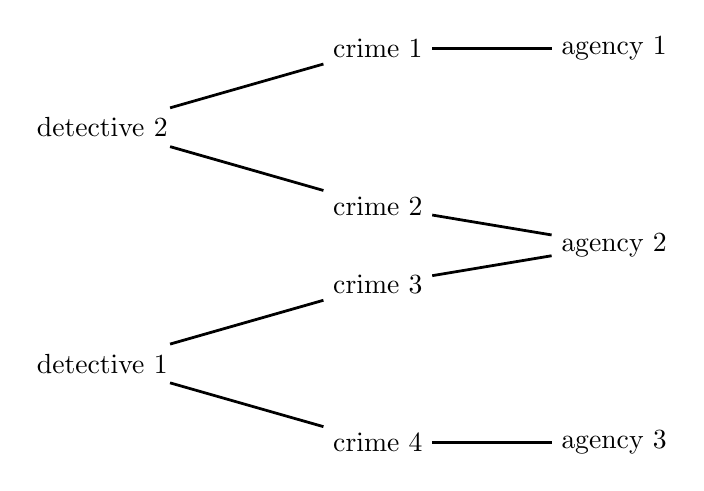
\begin{tikzpicture}[scale = \scale, baseline = {([yshift={-\ht\strutbox}]current bounding box.north)}]
\node (v1) at (2.5,2.5) {agency 1};
\node (v2) at (-0.5,2.5) {crime 1};
\node (v4) at (-0.5,0.5) {crime 2};

\node (v5) at (2.5,0) {agency 2};
\node (v6) at (-0.5,-0.5) {crime 3};
\node (v7) at (2.5,-2.5) {agency 3};
\node (v8) at (-0.5,-2.5) {crime 4};
\node (v3) at (-4,1.5) {detective 2};
\node (v9) at (-4,-1.5) {detective 1};
\draw [line width  = 1pt] (v2) edge (v1);
\draw [line width  = 1pt] (v4) edge (v5);
\draw [line width  = 1pt] (v6) edge (v5);
\draw [line width  = 1pt] (v8) edge (v7);
\draw [line width  = 1pt] (v9) edge (v6);
\draw [line width  = 1pt] (v9) edge (v8);
\draw [line width  = 1pt] (v4) edge (v3);
\draw [line width  = 1pt] (v3) edge (v2);
\end{tikzpicture}
\xe
%
Symmetric paraphrases:

\pex
\a 
Exactly two detectives each reported exactly two crimes to agencies\\
To exactly three agencies did detectives report exactly two crimes\\
\a 
Exactly two detectives each reported exactly two crimes to agencies\\
To exactly three agencies did detectives report exactly two crimes\\
\xe
%
\begin{squ}
The sentence is true because there is exactly one agency that detectives reported exactly two crimes for.
\end{squ}
%
However, it seems that this symmetric paraphrase is missing the \emph{each} operator that yields the correct reading. Not sure that Schein's argument goes through once we reestablish that:

\pex
\a 
Exactly two detectives each reported exactly two crimes to agencies\\
To exactly three agencies did detectives \textbf{each} report exactly two crimes\\
\a 
Exactly two detectives each reported exactly two crimes to agencies\\
To exactly three agencies did detectives \textbf{each} report exactly two crimes\\
\xe
%
In a later section, Schein spells out what seems to me to be a different, and I think better argument for symmetric logical forms. 

The idea is that symmetric logical forms overgenerate readings. In particular, if both quantifiers that enter the cumulative relationship are interpreted distributively in the logical formula:

\ex
Exactly two detectives each solved exactly two crimes for agencies \emph{and}\\
Exactly two agencies are each such that detectives solved crimes for them
\xe
%
Here, to verify the sentence under the reading: we need to find two crimes per agencies and two crimes per detectives. But the crimes solved for the agencies need not correspond to the crimes solved by the detectives one-to-one:

\ex
%!TEX root = ../plurals_event_chap_9.tex
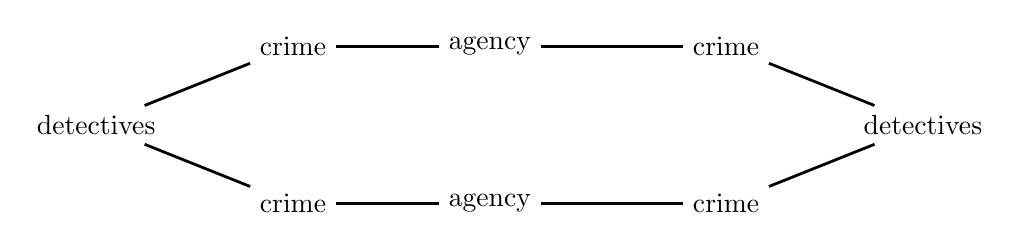
\begin{tikzpicture}[scale = \scale, baseline = {([yshift={-\ht\strutbox}]current bounding box.north)}]


\node (v1) at (-5,-0.5) {detectives};
\node (v2) at (-2.5,0.5) {crime};
\node (v3) at (-2.5,-1.5) {crime};
\node (v4) at (0,0.5) {agency};
\node (v8) at (0,-1.5) {agency};

\node (v5) at (3,0.5) {crime};
\node (v7) at (3,-1.5) {crime};

\node (v6) at (5.5,-0.5) {detectives};
\draw [line width = 1pt] (v1) edge (v2);
\draw [line width = 1pt] (v1) edge (v3);
\draw [line width = 1pt] (v2) edge (v4);
\draw [line width = 1pt] (v4) edge (v5);
\draw [line width = 1pt] (v5) edge (v6);
\draw [line width = 1pt] (v6) edge (v7);
\draw [line width = 1pt] (v7) edge (v8);
\draw [line width = 1pt] (v3) edge (v8);
\end{tikzpicture}
\xe
%


\section{What is the reference of the event anaphor}

\paragraph{Analogy with anaphors}
Schein's paraphrase of cumulative sentences involves an event anaphor, depicted as \emph{there}. 

\pex
\a 
Less than two detectives reported less than 3 crimes. 
\a \textbf{Schein's paraphrase:}\\
\emph{
Less than two detectives reported crimes\\
and there, less than 3 crimes were reported
}
\xe
%
For this paraphrase to go through, it would seem that \emph{there} should refer to all the events of reporting crimes to agencies by detectives. How does \emph{there} get to refer to this particular sets of events?

Schein's interesting observation is that there is no difference between event anaphors and anaphors to individuals, so whatever we need to say about the former is whatever we need to say about the latter. In particular, the following parallel is telling:

\definecolor{darkorange}{HTML}{efc67c}
\definecolor{bluegray}{HTML}{b1d1ed}
\definecolor{purple}{HTML}{ba83c4}
\pex
\a 
{\color{darkorange!84!black} Less than 3 farmers} bought {\fg a donkey}.\\
{\color{purple!93!black} They} carried {\color{bluegray!93!black} less than 4 bags of oats}.
\a 
{\color{darkorange!84!black} Less than 3 farmers} {\fg $\exists e$} bought donkeys.\\
{\color{purple!93!black} There,} {\color{bluegray!93!black} less than four donkeys} were bought.
\xe
%
In particular, he notes that in cross-clausal subordination contexts, there seems to be a difference in the reading of the anaphor depending on the nature of the subordinator\footnote{This data point, if genuine, is an added dimension to the problem of weak/strong reading in anaphors. In particular, it shows a weak/strong ambiguity look-alike that is not dependent on the monotonicity of the \emph{anaphor}'s environment (contra Kanazawa).}.

\pex
\a 
Few farmers bought a donkey\ldots\\
\ldots they hitched them together to a mule train.\\
\emph{they refers to all the bought donkeys}
\a 
Every farmer bought a donkey\ldots\\
\ldots they hitched them together to a mule train.\\
\emph{they refers to a plurality of one bought donkey per farmer}
\xe
%
So quantifiers like \emph{few} seem to impose maximal readings of the anaphors and while \emph{every} delivers non-maximal readings. This difference is claimed to be observable in event anaphor cross-reference as well:

\pex
\a 
In ten minutes, every farmer fed a donkey.
\a 
Every farmer $\exists e$ fed a donkey.\\
There, farmers fed donkeys in ten minutes\\
\emph{there refers to an event plurality containing one event per farmer}
\xe
%
A minimal pair with \emph{few} is lacking in the book. If we construct it, I am not certain that the reading we get is teh exact counterpart of \clastx 
\ex
In ten minutes, few farmers fed a donkey.
\xe
%
Not looking for a minimal pair, we already know that for cumulative sentences, \emph{there} must refer to all the buying events by a farmer, confirming the maximality already observed:

\ex
{\color{darkorange!84!black} Less than 3 farmers} bought {\fg a donkey}.\\
{\color{purple!93!black} They} carried {\color{bluegray!93!black} less than 4 bags of oats}.
\xe

\paragraph{Meandering aimlessly.} Schein get a bit stuck in his paraphrases because he is regrettably married to the idea that anaphors must be resolved as definite descriptions. 

\pex
{\bg Exactly two farmers}\textsubscript{56} each fed {\fg two donkeys}\textsubscript{89} {\color{purple} one bag of oats}\textsubscript{32}.\\
\a 
they\textsubscript{89} $\neq$ \emph{the donkeys that farmers fed bags of oats to}\\
they\textsubscript{89} $\neq$ \emph{the donkeys that the farmers fed one bag of oats to}
\a 
%!TEX root = ../plurals_event_chap_9.tex
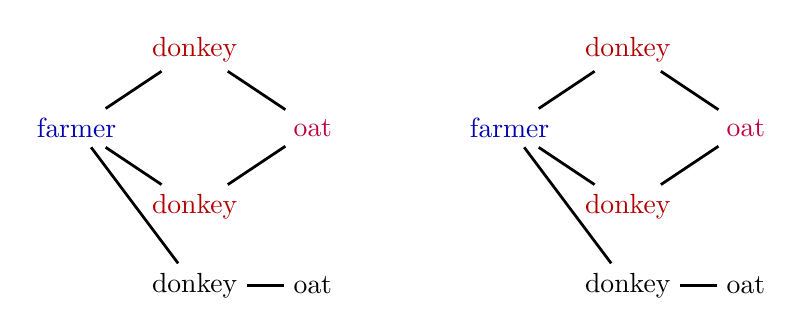
\begin{tikzpicture}[scale = \scale, baseline = {([yshift={-\ht\strutbox}]current bounding box.north)}]
\node (v2) at (-3,1.5) {\fg donkey};
\node (v3) at (-3,-0.5) {\fg donkey};
\node (v5) at (-1.5,0.5) {\color{purple} oat};
\node (v7) at (1,0.5) {\bg farmer};
\node (v8) at (2.5,1.5) {\fg donkey};
\node (v9) at (2.5,-0.5) {\fg donkey};
\node (v10) at (4,0.5) {\color{purple} oat};
\node (v1) at (-4.5,0.5) {\bg farmer};

\node (v4) at (-3,-1.5) {donkey};
\node (v6) at (-1.5,-1.5) {oat};
\node (v11) at (2.5,-1.5) {donkey};
\node (v12) at (4,-1.5) {oat};

\draw [line width = 1pt] (v1) edge (v2);
\draw [line width = 1pt] (v1) edge (v3);
\draw [line width = 1pt] (v1) edge (v4);
\draw [line width = 1pt] (v3) edge (v5);
\draw [line width = 1pt] (v2) edge (v5);
\draw [line width = 1pt] (v4) edge (v6);
\draw [line width = 1pt] (v7) edge (v8);
\draw [line width = 1pt] (v7) edge (v9);
\draw [line width = 1pt] (v8) edge (v10);
\draw [line width = 1pt] (v9) edge (v10);
\draw [line width = 1pt] (v7) edge (v11);
\draw [line width = 1pt] (v12) edge (v11);
\end{tikzpicture}
\xe
%
The correct definite descriptions are undesirable for Schein:

\begin{squ}
There ought to be more to the explanation of cumulative reference than an algorithm that introduces indefinite descriptions ad hoc into an already elaborate notion of descriptive content.
\end{squ}

\section{Rendering}

The solution is to adapt some vehicle for discourse referents, some entity which can hold all the entities that need to be transmitted to the next clause. Schein could have chosen assignments as in DS, or situations as in Heim/Elbourne E-type  theories. He chooses naturally to make events his DR vehicle\footnote{He calls his vehicle \emph{states of affair}, borrowing from Barry Taylor.} This is called \emph{rendering}: $E$ render a sentence $S$ if $E$ is the DR vehicle made available by $S$

Just as DS defines CCPs in a lexicalized manner, Schein defines for each operator in his logical formulas, the DR event that it introduces (i.e. the event that it renders). Here are some definitions:

\ex
\begin{tabular}[t]{ll}
  E renders $\Theta (X, E')$
  \\
  \emph{iff}
  \\
  $E$ is the set of events whose $\Theta$ is X\footnotemark
\end{tabular} 
\footnotetext{
I'm suppressing reference to complete overlap for simplicity (cf chap 4).
}
\xe
%
\ex~
\begin{tabular}[t]{ll}
E renders $Q x: \Phi(x), \Psi(x)$
\\
\emph{iff}
\\
$E= \left\lbrace e\text{ renders }\Psi(x)\ \middle|\ x\in\Phi\right\rbrace$
\end{tabular} 
\xe
%
\ex~ \label{exist}
\begin{tabular}[t]{ll}
E renders $\exists E: \Phi(E), \Psi(E)$
\\
\emph{iff}
\\
$E\in \Phi\cap\Psi$
\end{tabular} 
\xe
%
The latter two denotations are close relatives with the corresponding DS denotation. For quantifiers, the DRs introduced in each true quantificational case are gathered together in one big DR ; for existentials, any witness would do. With this, we are ready to confront the donkey problem seen earlier:

\pex
{\bg Exactly two farmers}\textsubscript{56} each fed {\fg two donkeys}\textsubscript{89} {\color{purple} one bag of oats}\textsubscript{32}.
\a 
\begin{tabular}[t]{ll}
they\textsubscript{89} & $\neq$ \emph{the donkeys that the farmers fed one bag of oats to}\\
 & $=$ \emph{the theme donkeys in the events that render \cnextxa}
\end{tabular}
\a 
%!TEX root = ../plurals_event_chap_9.tex
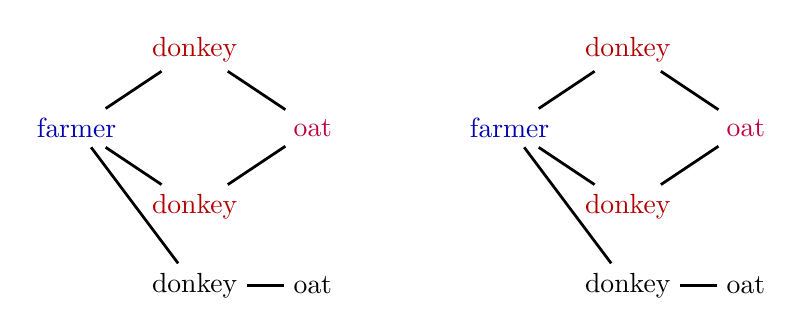
\begin{tikzpicture}[scale = \scale, baseline = {([yshift={-\ht\strutbox}]current bounding box.north)}]
\node (v2) at (-3,1.5) {\fg donkey};
\node (v3) at (-3,-0.5) {\fg donkey};
\node (v5) at (-1.5,0.5) {\color{purple} oat};
\node (v7) at (1,0.5) {\bg farmer};
\node (v8) at (2.5,1.5) {\fg donkey};
\node (v9) at (2.5,-0.5) {\fg donkey};
\node (v10) at (4,0.5) {\color{purple} oat};
\node (v1) at (-4.5,0.5) {\bg farmer};

\node (v4) at (-3,-1.5) {donkey};
\node (v6) at (-1.5,-1.5) {oat};
\node (v11) at (2.5,-1.5) {donkey};
\node (v12) at (4,-1.5) {oat};

\draw [line width = 1pt] (v1) edge (v2);
\draw [line width = 1pt] (v1) edge (v3);
\draw [line width = 1pt] (v1) edge (v4);
\draw [line width = 1pt] (v3) edge (v5);
\draw [line width = 1pt] (v2) edge (v5);
\draw [line width = 1pt] (v4) edge (v6);
\draw [line width = 1pt] (v7) edge (v8);
\draw [line width = 1pt] (v7) edge (v9);
\draw [line width = 1pt] (v8) edge (v10);
\draw [line width = 1pt] (v9) edge (v10);
\draw [line width = 1pt] (v7) edge (v11);
\draw [line width = 1pt] (v12) edge (v11);
\end{tikzpicture}
\xe
%
Note that Schein is still married to E-type descriptions. He gives one reason why: definite descriptions introduce maximality, which Evans argues is desirable for definite descriptions.

\pex
\a John owns some sheep\textsubscript{63}.
\a Harry vaccinated them\textsubscript{63}.
\xe
%
By the denotation in \cref{exist}, the events that render \clastxa true are any events of John owning sheep.  The definite description in \clastxb will only pick out the maximal event that renders \clastxa true. This way, we ensure that all the sheep owned by John were vaccinated. This is a different division of labor than is usually found in DS. In DS, maximality is introduced at the level of the pronoun rather than its antecedent\footnote{Difficult to know whether this is preferable to the DS way of doing things. If we adopt a Heim (1982, chap 1) way of doing donkey sentences, then the sentence in \cnextxa may be predicted to have the reading in \cnextxb if maximality is only introduced at the level of the pronoun.

\pex
\a 
Every farmer who owns donkeys drew a circle around them\\
\a 
Drew a circle around each subgroup of donkeys.
\xe
%
But there may be other ways of doing donkeys with Schein's tools.
}.

\paragraph{DE quantifiers.} Downward entailing quantifiers are compatible with a situation with no witness, hence no rendering event. Yet, that does not result in problematic truth-conditions.

\pex
\a 
Less than 3 detectives each solved exactly two crimes for less than three agencies.
\a 
\textbf{Schein's paraphrases:}\\
\emph{[less than 3 detectives solved exactly two crimes for agencies]\textsubscript{78}}\\
\emph{there\textsubscript{78}, detectives each solved exactly two crimes for less than three agencies}
\xe
%
Indeed, in the context of \cnextx, the clause 78 is rendered by the empty event (no detectives solved exactly two crimes). So it is true that for less than three agencies, exactly two crimes were solved.

\ex
%!TEX root = ../plurals_event_chap_9.tex
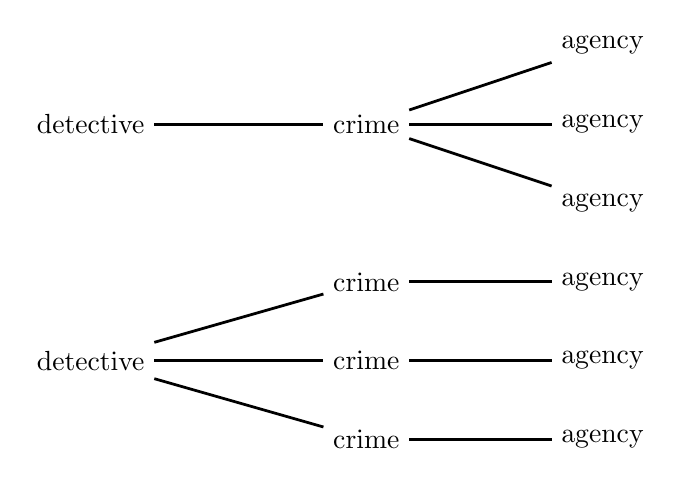
\begin{tikzpicture}[scale = \scale, baseline = {([yshift={-\ht\strutbox}]current bounding box.north)}]

\node (v3) at (2.5,2.5) {agency};
\node (v12) at (2.5,0.5) {agency};
\node (v6) at (2.5,-0.5) {agency};
\node (v8) at (2.5,-1.5) {agency};
\node (v10) at (2.5,-2.5) {agency};
\node (v4) at (2.5,1.5) {agency};

\node (v2) at (-0.5,1.5) {crime};
\node (v5) at (-0.5,-0.5) {crime};
\node (v7) at (-0.5,-1.5) {crime};
\node (v9) at (-0.5,-2.5) {crime};

\node (v1) at (-4,1.5) {detective};
\node (v11) at (-4,-1.5) {detective};



\draw [line width = 1pt] (v2) edge (v3);
\draw [line width = 1pt] (v2) edge (v4);
\draw [line width = 1pt] (v5) edge (v6);
\draw [line width = 1pt] (v7) edge (v8);
\draw [line width = 1pt] (v9) edge (v10);
\draw [line width = 1pt] (v11) edge (v5);
\draw [line width = 1pt] (v11) edge (v7);
\draw [line width = 1pt] (v11) edge (v9);
\draw [line width = 1pt] (v1) edge (v2);
\draw [line width = 1pt] (v2) edge (v12);

\end{tikzpicture}
\xe
%
But there is a problem in the lurking with DE quantifiers, if the quantifier that does not enter the cumulative relation is a DE quantifier, as in \cnextx:

\pex
\a 
Exactly two detectives solved no crimes for exactly two agencies
\a 
\textbf{Schein's paraphrases:}\\
\emph{[exactly two detectives solved solved no crimes for agencies]\textsubscript{78}}\\
\emph{there\textsubscript{78}, detectives each solved crimes for exactly two agencies}
\xe
%
Here, no event renders clause 78. So the second clause is falsified, no matter what the actual context is like. Schein reports his solution to a later stage.

To reassure the reader though, he just notes in \cnextx that DE quantifiers do indeed antecede ordinary pronouns, without introducing $\exists$ inference. So even Schein's modeling of anaphoric dependencies need to be modified, there is hope that some solution is possible.

\ex
Few\textsubscript{89} senators voted for JFK and they\textsubscript{89} supported all Democrats' bills.
\xe
%
Schein believes this does not imply the existence of anyone voting for JFK. I'm not so certain:

\ex
I bet that few senators will vote for JFK and they will support all Democrats' bills.
\xe
%

\section{Cumulative readings may be symmetric}

\paragraph{Symmetric readings.}
After convincing us that cumulative readings are by nature asymmetric, Schein considers an exception which he attributes to May, given in \cnextxa. In this reading, {\fg red} arguments enter a cumulative relation and the {\bg blue} argument is interpreted distributively wrt both of them.

\pex
\a 
{\fg Two officials} sold {\bg two secret documents} to {\fg two superpowers}.\label{symmetric}
\a 
Gather all pairs $(x, y)$ of official-super power such that $x$ sold two secret documents to $y$\\
These pairs must involve two officials and two superpowers
\xe
%
Note that this sentence comes very close in meaning to the sentences we used to evidence asymmetric reading repeated in \cnextx. In the asymmetric reading, the {\bg blue} argument is only distributive wrt the subject

\ex
{\fg Less than 3 detectives} each solved {\bg exactly two crimes} for {\fg less than three agencies}.
\xe
%
Schein notes that symmetric readings are problematic for his asymmetric LFs. For instance, the scenario depicted in \cnextxc falsifies the symmetric reading but verifies the asymmetric LF that Schein would assign \cref{symmetric}, paraphrased in \cnextxb:

\pex
\a 
{\fg Two officials} sold {\bg two secret documents} to {\fg two superpowers}.\label{symmetric}
\a
Two officials sold two secret documents each to two super-powers \emph{and}\\
There, to two super-powers were two secret documents each sold
\a 
%!TEX root = ../plurals_event_chap_9.tex
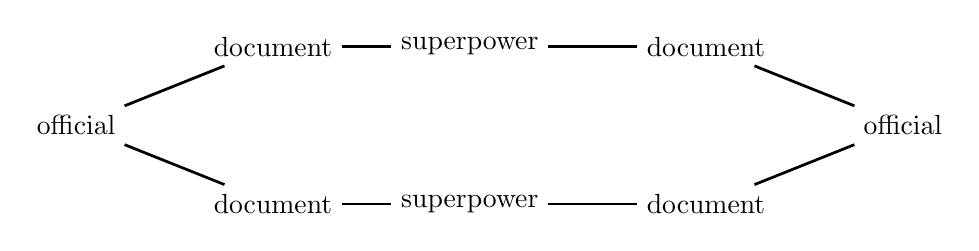
\begin{tikzpicture}[scale = \scale, baseline = {([yshift={-\ht\strutbox}]current bounding box.north)}]

\node (v1) at (-5,-0.5) {official};
\node (v2) at (-2.5,0.5) {document};
\node (v3) at (-2.5,-1.5) {document};
\node (v4) at (0,0.5) {superpower};
\node (v8) at (0,-1.5) {superpower};

\node (v5) at (3,0.5) {document};
\node (v7) at (3,-1.5) {document};

\node (v6) at (5.5,-0.5) {official};
\draw [line width = 1pt] (v1) edge (v2);
\draw [line width = 1pt] (v1) edge (v3);
\draw [line width = 1pt] (v2) edge (v4);
\draw [line width = 1pt] (v4) edge (v5);
\draw [line width = 1pt] (v5) edge (v6);
\draw [line width = 1pt] (v6) edge (v7);
\draw [line width = 1pt] (v7) edge (v8);
\draw [line width = 1pt] (v3) edge (v8);
\end{tikzpicture}
\xe
%
Schein is vague on this point but I don't know the doubly-distributive reading he does that he predicts is present.

\paragraph{Reason for skepticism.} 
Acknowledging these readings might lead us to an analysis with a binary quantifier over pairs, as May recommended.

However, Schein has reasons to be skeptical. He finds that the target reading is not as easily available in all configurations.
He finds the reading unobjectionable if the {\bg blue} argument is an increasing quantifier but the reading for the non-increasing quantifier, he judges to be contrived.

\pex
\a 
\ljudge? {\fg Two officials} sold {\bg no more than six documents} to {\fg two superpowers}
\a 
\ljudge? {\fg Two officials} sold {\bg no documents} to {\fg two superpowers}
\xe
%
This is motivation to pursue a new analysis in terms of the asymmetric analysis we have been assuming so far

\paragraph{Pragmatic solution: contexts of events.} Schein first proposes that May's readings may come about when the context only makes available events where one official sells to one superpower. In other words, the only events made available in the context considered above would be the one circled in \cnextx:

\ex
%!TEX root = ../plurals_event_chap_9.tex
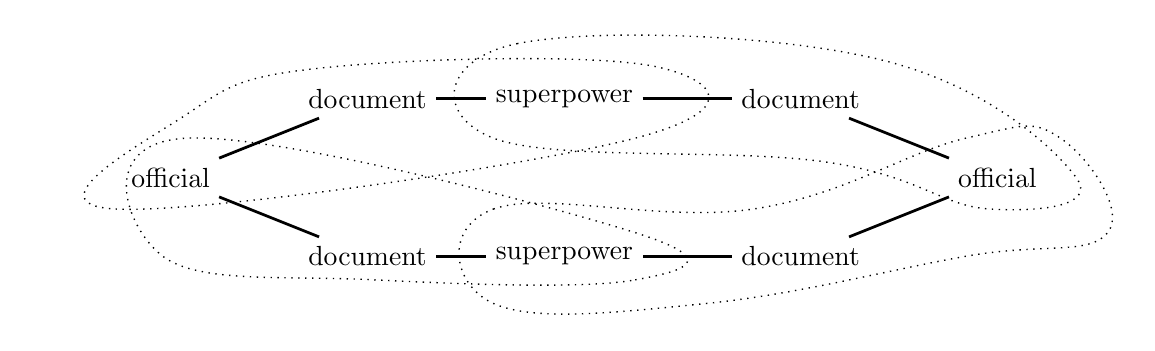
\begin{tikzpicture}[scale = \scale, baseline = {([yshift={-\ht\strutbox}]current bounding box.north)}]


\node (v1) at (-5,-0.5) {official};
\node (v2) at (-2.5,0.5) {document};
\node (v3) at (-2.5,-1.5) {document};
\node (v4) at (0,0.5) {superpower};
\node (v8) at (0,-1.5) {superpower};

\node (v5) at (3,0.5) {document};
\node (v7) at (3,-1.5) {document};

\node (v6) at (5.5,-0.5) {official};
\draw [line width = 1pt] (v1) edge (v2);
\draw [line width = 1pt] (v1) edge (v3);
\draw [line width = 1pt] (v2) edge (v4);
\draw [line width = 1pt] (v4) edge (v5);
\draw [line width = 1pt] (v5) edge (v6);
\draw [line width = 1pt] (v6) edge (v7);
\draw [line width = 1pt] (v7) edge (v8);
\draw [line width = 1pt] (v3) edge (v8);
\draw [dotted, line width = 0.5pt] plot[smooth cycle, tension=.7] coordinates {(-4.8,0.3) (-5.7,-0.9) (0.9,0) (1.2,0.9) (-3,0.9)};
\draw [dotted, line width = 0.5pt] plot[smooth cycle, tension=.7] coordinates {(-2.4,-1.8) (0.9,-1.8) (0.9,-1.2) (-4.8,0) (-5.1,-1.5)};
\draw [dotted, line width = 0.5pt] plot[smooth cycle, tension=.7] coordinates {(-0.9,0) (-0.6,1.2) (4,1) (6.5,-0.5) (5.4,-0.9) (3.3,-0.3)};
\draw [dotted, line width = 0.5pt] plot[smooth cycle, tension=.7] coordinates {(-0.9,-2.1) (-0.9,-0.9) (2.4,-0.9) (5.1,0) (6.3,0) (6.9,-1.2) (5.1,-1.5) (1.8,-2.1)};
\end{tikzpicture}
\xe
%
With this restriction on the set of events, 
The asymmetric paraphrase in \cnextxb correctly falsifies \cnextxa:

\ex
For each of two officials $x$, there is an event \underline{in the context} where $x$ sells two secret documents to super-powers \emph{and}
There, two super-powers were sold documents to
\xe
%
It seems that Schein has taken liberties with the logical formulas to derive this resuit:

\begin{itemize}
\item \emph{two officials} scopes above event closure.
\item \emph{two secret documents} is not repeated in the pronominal clause.
\end{itemize}
%
But since he will end up adopting a different analysis, let's look past that\footnote{
I am also missing part of the reasoning there. Schein presents a problem to this analysis, which I don't think arises and proceeds to solve it. His solution however, does not seem to change anything to the logical formula used
}. 

\paragraph{Solution II: semantic solution.}
Schein proposes an alternative purely semantic solution. So far, the cumulative logical formula involved a first conjunct which contained all but one of the quantifiers, the other quantifiers being replaced with low-scoping existentials. This conjunct served as antecedent

\pex
\a
{\fg Two officials} sold two documents to {\bg super-powers} \emph{and}\\
Two superpowers were sold two documents
\a
$\exists X : 2\text{ officials}, \forall x\in X, \exists Y : \text{super-powers},\ x$ sold documents to $y$ $\wedge$
\ldots
\xe
%
However, Schein notes the we do not have to interpret the {\bg blue} quantifier \emph{in situ} necessarily. In particular, as we've seen in previous chapters, we can scope {\bg super-powers} and interpret it distributively in the first conjunct. That seems enough for May's reading.

\pex
\a
Two officials are each such that superpowers each received two documents from them.\\
There, to two superpowers were documents sold.
\a
$\exists X : 2\text{ officials}, \forall x\in X, \exists Y : \text{super-powers}, \underline{\forall y\in Y},\ x$ sold two documents to $y$ $\wedge$\ldots
\xe
%

\paragraph{Back to decreasing quantifiers.}
Earlier, Schein observed that May's readings were possible but degraded.

\pex
\a 
\ljudge? {\fg Two officials} sold {\bg no more than six documents} to {\fg two superpowers}
\a 
\ljudge? {\fg Two officials} sold {\bg no documents} to {\fg two superpowers}
\xe
%
Under the asymmetric logical formula that Schein gives these sentences, cross-reference to events should fail. Negative events do not introduce referents.

\ex
$\exists X : 2\text{ officials}, \forall x\in X, \exists Y : \text{super-powers}, \forall y\in Y,\ x$ sold no documents to $y$ $\wedge$\ldots
\xe
%
However, reference may be possible if the event existential which introduces event referents outscopes negation. That is to say, if the reference is to negative events. We can now tie the oddness of the sentence to the oddness of negative events:

\ex
$\exists X : 2\text{ officials}, \forall x\in X, \exists Y : \text{super-powers}, \forall y\in Y, \exists E, x$ sold no documents to $y$ $\wedge$\ldots
\xe
%


\section{Syntactic constraints on cumulative readings}

Schein observes (foreshadowing Beck \& Sauerland) that cumulative readings are not tied to single clause contexts:

\ex
No more than two detectives found solutions to no more than two problems.
\xe
%
Schein's observation is that the pronominal clauses in his paraphrase will have to copy everything from both clauses:

\ex
No more than two detectives found solutions to problems \emph{and}\\
To no more than two problems did detectives find solutions.
\xe
%
I'm skipping much of the discussion of the biclausal cases that I didn't find particularly interesting

\paragraph{Constraints on cumulative readings.}
This is more interesting. Schein notes that adjuncts display an ambiguity in their cumulative readings.

\pex
Less than three people died because of less than five good samaritans.
\a 
\textbf{Cumulative Interpretation:} \emph{the number of casualties by good samaritans was less than 3 and less than 5 good samaritans occasioned casualties}
\a 
\textbf{\quo{Separated} interpretation:} \emph{the deah toll was less than 3 and less than 5 good samaritans made that outcome possible}
\xe
%
I note that extraposition of the adjunct leads to an unmistakable \quo{separated interpretation}:

\ex
Less than three people died yesterday, because of less than 5 good samaritans.
\xe
%
The separated interpretation seems to arise in Schein's system when each quantifier can QR within its own domain. When they do, no qunatifier takes scope above the other ; yet, this is not a cumulative reading as the two quantifiers do not have the same scope: each lives in its own domain.

\pex
\a 
\textbf{Cumulative interpretation:}\\
\Tikzmark{end1}{} \hspace{5ex} \Tikzmark{beg2}{Less than 3 people} died because of \Tikzmark{beg1}{less than 5 good samaritans}.\\[2ex]
\DrawArrow{beg1}{end1}{below}{} % [tikz options-]beginning-end-position-text[- distance to line]
\DrawArrow{beg2}{end1}{below}{}[2.5] % [tikz options-]beginning-end-position-text[- distance to line]
\a \textbf{Separated interpretaion:}\\
\Tikzmark{end2}{\hphantom{a}} \hspace{5ex} \Tikzmark{beg2}{Less than 3 people} died \Tikzmark{end1}{\hphantom{a}} because of \Tikzmark{beg1}{less than 5 good samaritans}.\\[2ex]
\DrawArrow{beg1}{end1}{below}{} % [tikz options-]beginning-end-position-text[- distance to line]
\DrawArrow{beg2}{end2}{below}{} % [tikz options-]beginning-end-position-text[- distance to line]
\xe
%


The possibility of extraposition (which Schein confusingly calls \emph{separation}) diagnoses the presence of a syntactic domain in which QR may land, infers Schein. So if an argument finds itself in an extraposable domain where the other argument isn't, a separated interpretation is possible.

To prove this in greater details, Schein constructs a number of examples in which extraposition is impossible and a cumulative reading is contradictory. He finds that in such sentences, only a distributive interpretation is possible:

\pex Impossible extraposition
 \a 
 Few boys gave girls no nice roses
 \a 
 \textbf{Impossible separated reading:} \emph{Few boys gave girls anything. And they gave them no nice roses.}
 \xe
 %
\pex~ Possible extraposition
\a 
Few boys gave roses to no nice girls.
\a 
 \textbf{Possible separated reading:} \emph{Few boys gave roses to anyone. And they gave them to no nice roses.}
\xe
%
(I think an intonational break is required for these examples)



\end{document}
